
\begin{frame}{Realidad Aumentada (AR) \footnotemark}
%\begin{block}{Realidad Aumentada (AR) \footnotemark} 
\begin{columns}
\begin{column}{0.49\textwidth}
\begin{itemize}
\item La AR es una experiencia que traslapa elementos digitales (modelados por computadora) con el mundo físico del usuario (adquirido mediante una cámara). 
\item Los elementos digitales se combinan con las vistas del mundo real.
\end{itemize}
\end{column}
\begin{column}{0.49\textwidth}
\begin{center}
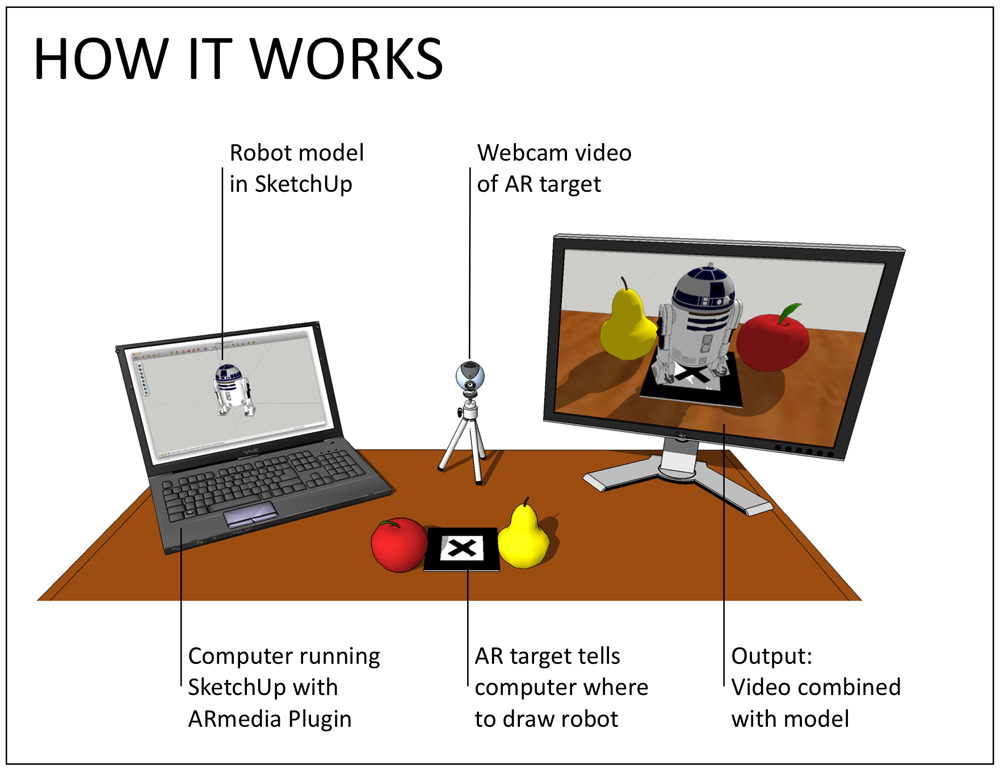
\includegraphics[width=0.95\textwidth]{Figs/AR_HowItWorks}
\end{center}
\end{column}
\end{columns}
\footnotetext{\url{http://photos1.blogger.com/img/m-a310d3b7b46f285189e1d6da63a1afd13be4ffc4.jpg}}
%\end{block} 
\end{frame}

\begin{frame}{Pasos en la detección de marcadores de AR \footnotemark}
%\begin{block}{Pasos en la detección de marcadores de AR \footnotemark} 
\begin{columns}
\begin{column}{0.39\textwidth}
\begin{enumerate}
\item Umbralización.
\item Detección del Marcador.
\item Estimación de Pose y Posición.
\item Empalme del modelo 3D.
\end{enumerate}
\end{column}
\begin{column}{0.59\textwidth}
\begin{center}
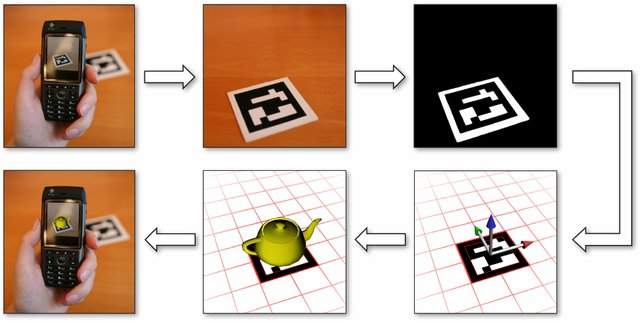
\includegraphics[width=0.95\textwidth]{Figs/AR_WorkFlow}
\end{center}
\end{column}
\end{columns}
%\end{block} 
\footnotetext{\fullcite{Wagner_ArToolKitPlus2007}}
\end{frame}


\begin{frame}{Tipos de Aplicación de AR \footnotemark}
%\begin{block}{Tipos de Aplicación de AR \footnotemark} 
\begin{columns}
\begin{column}{0.98\textwidth}
    \begin{center}

\begin{itemize}
\item Basadas en Localización. Están basada en sensores GPS para determinar la ubicación del dispositivo para crear objetos AR
\item Basadas en Visión – Utilizan una cámara, aunque también es posible incorporar sensores (compass, acelerómetros, giroscopios, etc). 
\begin{itemize}
\item  Requieren Marcadores (Marker) – Localizan un patrón o marcador QR  y renderizan un objeto 3D basado en su localización en el espacio real. 
\item  No requieren marcadores (Markerless)– Se emplean esquinas y puntos característicos del espacio real
\end{itemize}
\end{itemize}
     \end{center}

\end{column}
\end{columns}
%\end{block} 
\footnotetext{\url{https://fswa-net.com/index.php/news/use-of-ar-technology}}

%\\setcounter{footnote}{0}
\end{frame}


\begin{frame}{Aplicaciones de RA}
%\begin{block}{Aplicaciones de RA} 
\begin{itemize}
\item Aplicaciones principales: Arquitectura, Cosméticos, Contenido social, Marketing, Juegos, etc
\end{itemize}

\begin{columns}
\begin{column}{0.49\textwidth}
\begin{itemize}
\item Houzz
\end{itemize}
\begin{center}
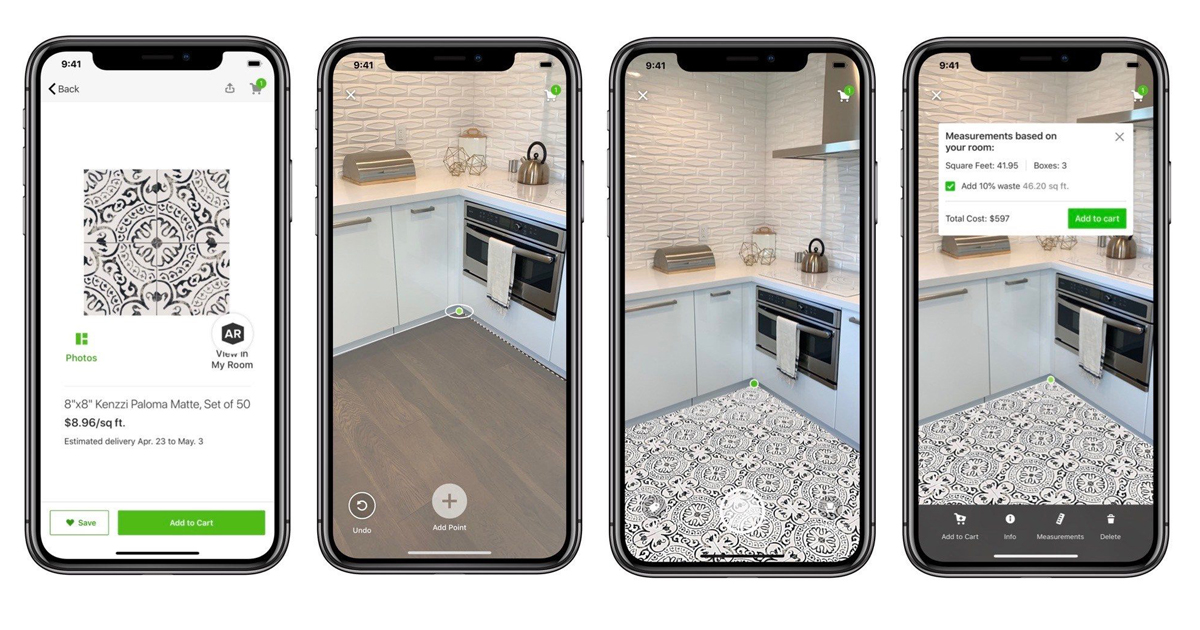
\includegraphics[width=0.9\textwidth]{Figs/AR_App}\\
\end{center}
\end{column}
\begin{column}{0.49\textwidth}  

\begin{itemize}
\item Pokemon Go
\end{itemize}
    \begin{center}
     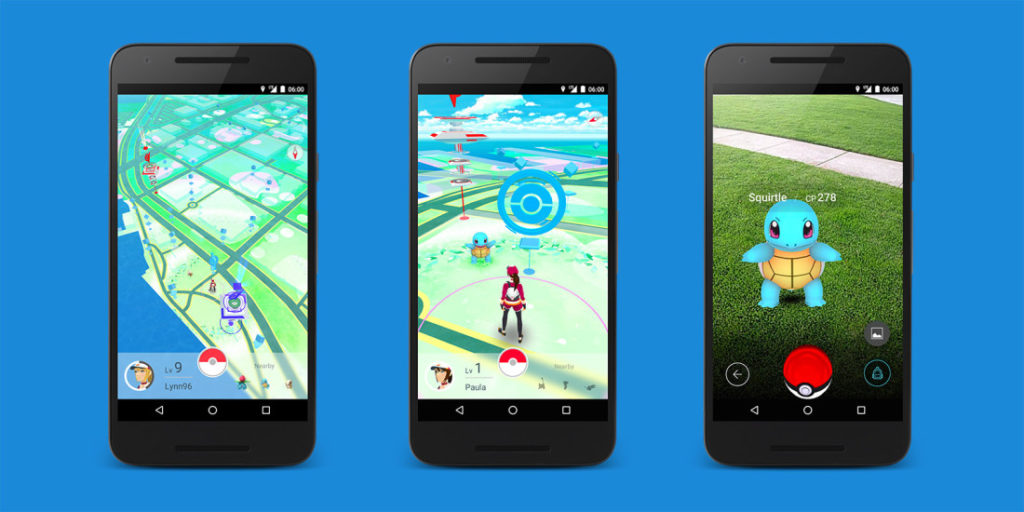
\includegraphics[width=0.9\textwidth]{Figs/Pokemon}
     \end{center}
\end{column}
\end{columns}
%\end{block} 
\end{frame}


\begin{frame}{Realidad Virtual - Antecedente hist\'orico}

\begin{columns}
\begin{column}{0.49\textwidth}


\begin{itemize}
\item Un estereoscopio proporciona im\'agenes separadas para cada ojo mediante lentes individuales, donde cada imagen tiene una variante en el angulo de captura y un desplazamiento horizontal.
\item El cerebro de una persona con una percepción binocular normal de la profundidad al utilizar el estereoscopio ``mezcla'' ambas imagenes para crear una  ``ventana estereoscópica''
\end{itemize}
\end{column}

\begin{column}{0.49\textwidth}

\begin{center}
	\begin{tabular}{cc}
        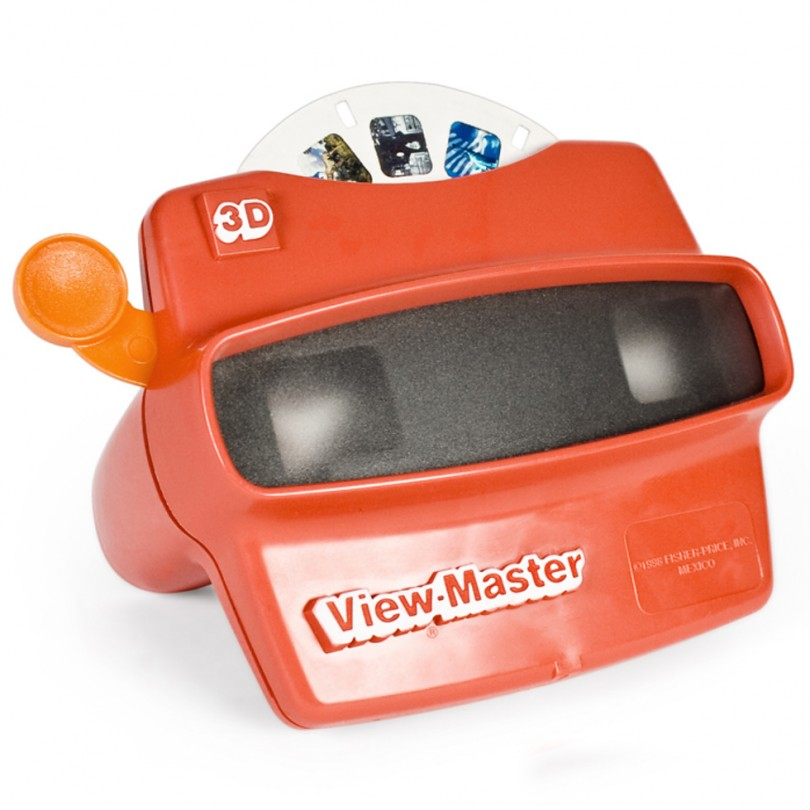
\includegraphics[width=0.45\linewidth]{Figs/view_master_blog-810x810.jpg} &
		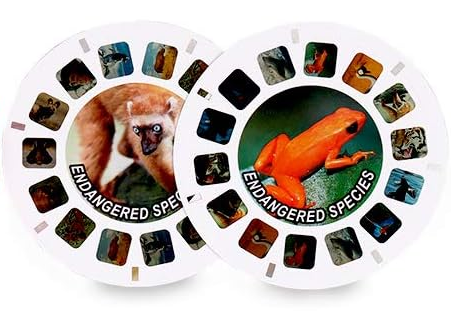
\includegraphics[width=0.45\linewidth]{Figs/DiscosViewMaster.png}    
	\end{tabular}

	\begin{tabular}{cc}
	\centering
        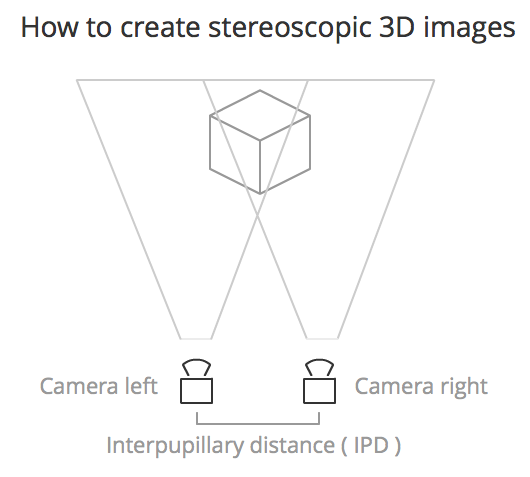
\includegraphics[width=0.49\linewidth]{Figs/VirtualReal1} &
        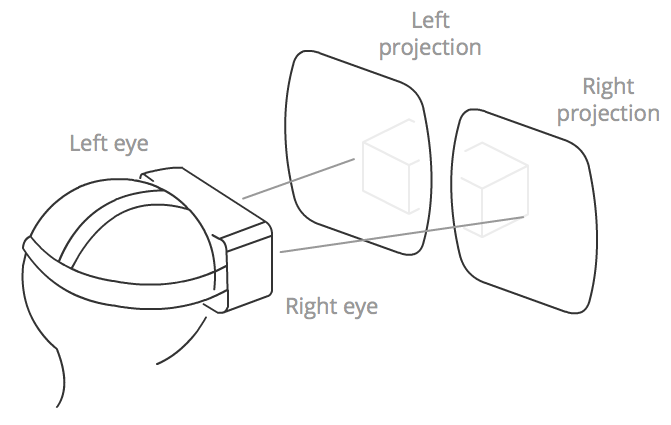
\includegraphics[width=0.49\linewidth]{Figs/VirtualReal2} \\

	\end{tabular}
\end{center}
\end{column}

\end{columns}

\end{frame}




\begin{frame}{Realidad Virtual (VR)}
%\begin{block}{Realidad Virtual (VR)} 
		\begin{itemize}
			\item La Realidad virtual (RV) emplea modelos y simulaciones por computadora que permite a una persona interactuar con un entorno visual artificial tridimensional (3D)
			\item En un formato típico de RV, un usuario lleva un casco con una pantalla estereoscópica para ver imágenes animadas de un entorno simulado
			\item El dispositivo m\'as econ\'omico para aplicaciones de RV es un tel\'efono inteligente 
		\end{itemize}
    \begin{center}
	\begin{tabular}{ccc}
    	\centering
		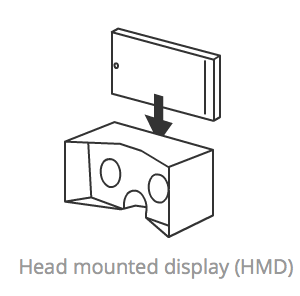
\includegraphics[width=0.25\linewidth]{Figs/MobileVR2} & 
        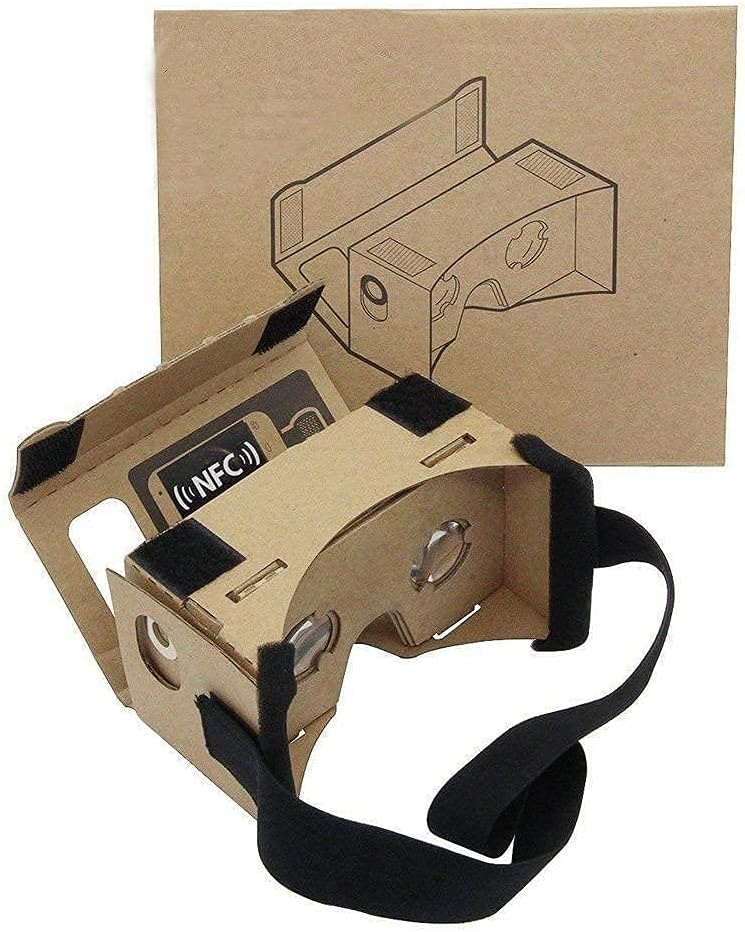
\includegraphics[width=0.19\linewidth]{Figs/CardBoard} & 		
        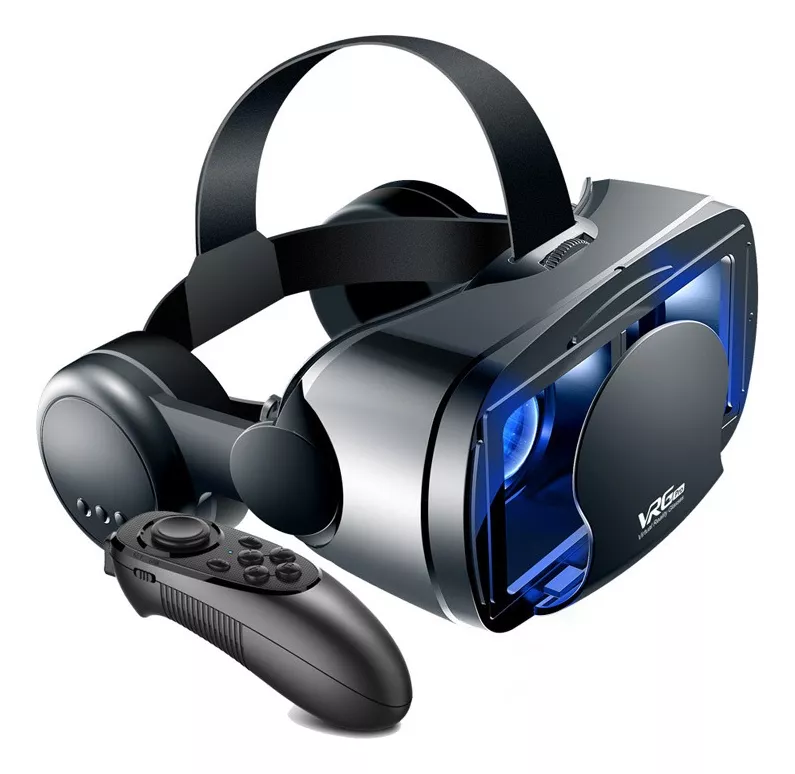
\includegraphics[width=0.19\linewidth]{Figs/VRGPro} 		
	\end{tabular}
		 \end{center}
%\end{block} 
\footnotetext{\url{https://reference.codeproject.com/book/dom/webvr_api/webvr_concepts}}
\end{frame}


\begin{frame}{Costos de Dispostivos HeadSets para VR}
\begin{columns}
\begin{column}{0.49\textwidth}
\begin{itemize}
\item Meta Quest 3 (499 USD)
\item Sony PlayStation VR2 (599 USD)
\item Meta Quest Pro (900 USD)
\item Valve Index VR Kit (1350 USD)
\item HTC Vive Pro 2 (1400 USD)
\end{itemize}

\begin{center}
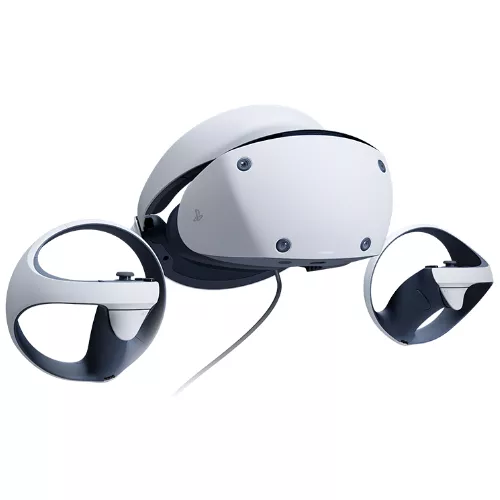
\includegraphics[width=0.75\textwidth]{Figs/sony.png}
\end{center}
\end{column}
\begin{column}{0.49\textwidth}
\begin{center}
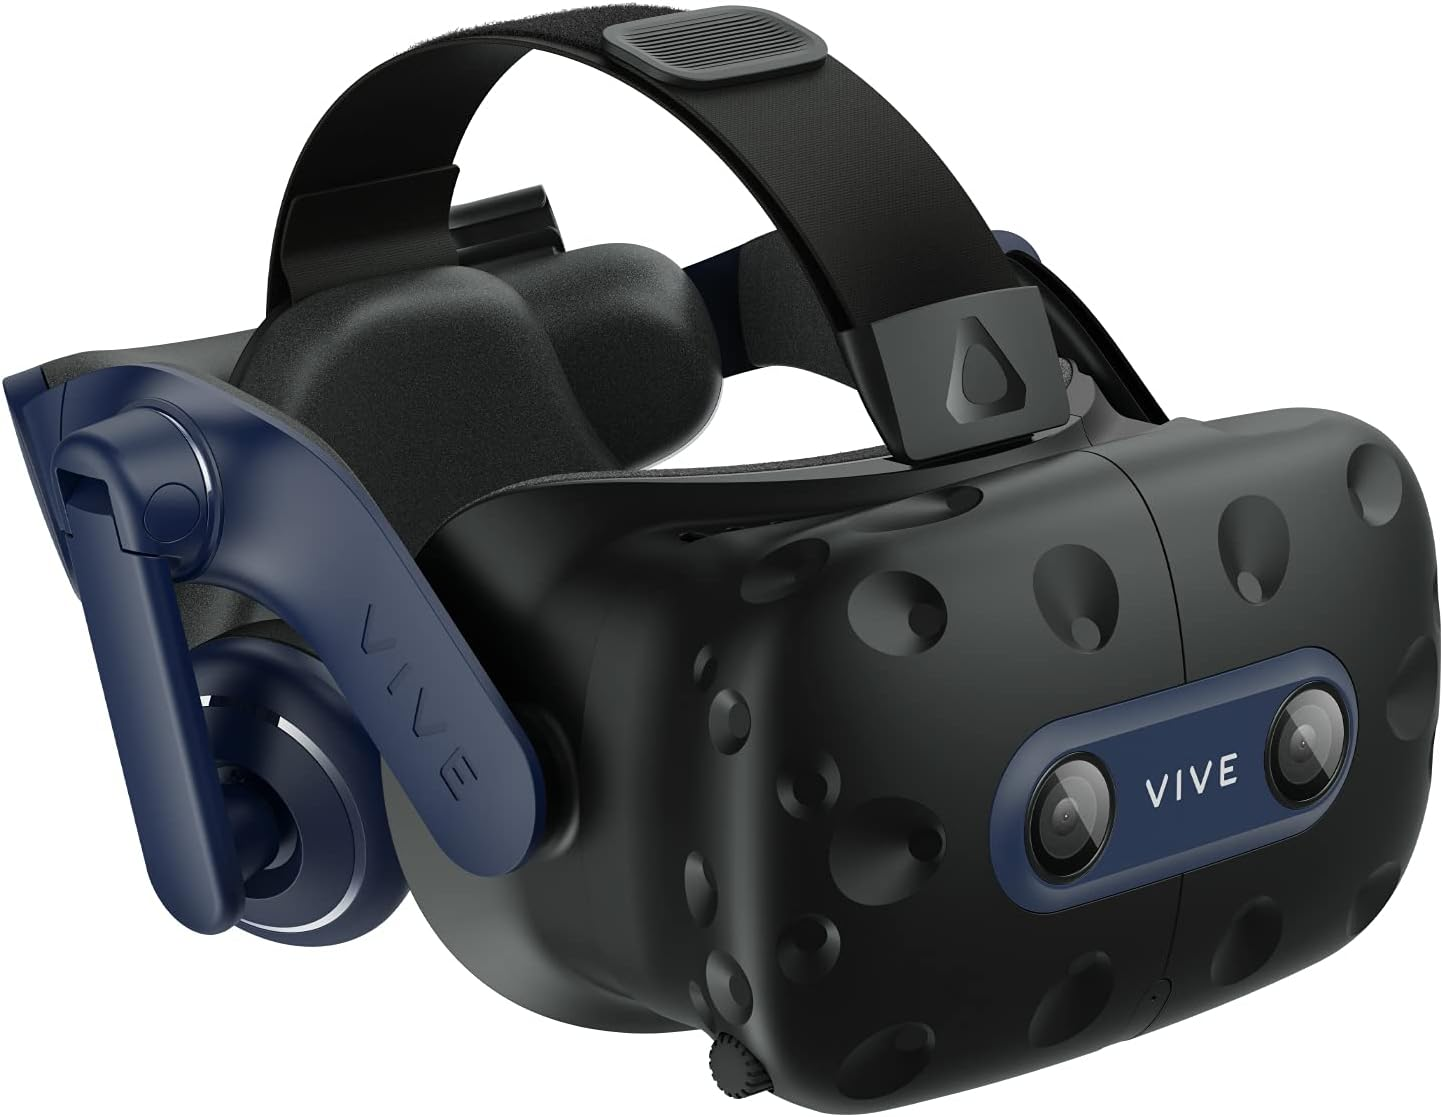
\includegraphics[width=0.75\textwidth]{Figs/HTC.jpg}\\
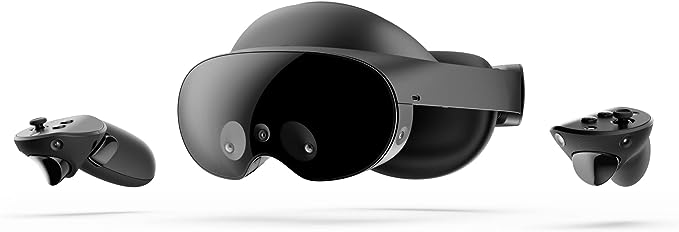
\includegraphics[width=0.95\textwidth]{Figs/MetaPro.jpg}
\end{center}
\end{column}
\end{columns}
\end{frame}
